\chapter{Practical Evaluation}

This practical evaluation has 2 main parts:
\begin{enumerate}
    \item an \texttt{afl} test run on a sample program with some intentional
    memory safety vulnerabilities that can be triggered by specially-crafted
    input files
    \item a very brief overview of some real-world bugs and vulnerabilities
    found by \texttt{afl} as well as its overall effect on the security
    community
\end{enumerate}

Note that the test program used in Section \ref{sec:my-fuzz} is contrived and
naively written, used only for demonstration purposes. It's important to
recognize that \texttt{afl} is well-suited, and, indeed, designed for, very
large and complex real-world programs, although it's certainly also applicable
to much smaller tools as well.

\section{Fuzzing a Toy Program}
\label{sec:my-fuzz}

\texttt{msg-parse} is a small C program that reads
message structures (as defined in Figure \ref{fig:msg}) into a buffer,
attempts to parse a message from the buffer, and then prints the
\texttt{addr} and \texttt{uname} fields. See Appendix \ref{app:vuln-full}
for full source code, and Appendix \ref{app:vuln-seed} for a tool that
will generate correct message structure files. \\

\begin{figure}[H]
    \begin{lstlisting}[language={[ANSI]C}]
typedef struct {
    uint8_t type;
    uint8_t addr_len;
    uint8_t uname_len;
    uint16_t len;
    char *addr;
    char *uname;
} msg_t;
\end{lstlisting}
\caption{Message stucture definition used in vulnerable program.}
\label{fig:msg}
\end{figure}

\subsection{The Vulnerable Code}

\texttt{msg-parse} has 3 vulnerabilities related to invalid memory reads
and writes, detailed in the code snippet in Figure \ref{fig:vuln-snippet}. \\

\begin{figure}[H]
    \begin{lstlisting}[language={[ANSI]C}]
// UNSAFE 1: read of buf[idx] without checking
//           idx+msg->addr_len < buf_len
memcpy(msg->addr, &(buf[idx]), msg->addr_len);
idx += msg->addr_len;
msg->addr[msg->addr_len] = '\0';

// UNSAFE 2: read of buf[idx] without checking
//           idx+msg->uname_len < buf_len
memcpy(msg->uname, &(buf[idx]), msg->uname_len);
msg->uname[msg->uname_len] = '\0';                                         

// for user privacy, zero-out message buffer
// when we're done with it
// UNSAFE 3: writes to buf without checking
//           msg->len <= buf_len
memset(buf, 0, msg->len);
\end{lstlisting}
\caption{A vulnerable code snippet that, when given malicious or malformed data, will violate memory safety.}
\label{fig:vuln-snippet}
\end{figure}

\subsection{\texttt{afl} Setup and Execution}

\texttt{msg-parse} was compile using the \texttt{afl-gcc} wrapper and
\texttt{ASAN}\footnote{https://github.com/google/sanitizers/wiki/AddressSanitizer}.
Figure \ref{fig:afl-build} shows the actual command used to build \texttt{msg-parse},
and Figure \ref{fig:afl-run} shows the command to start \texttt{afl-fuzz}, the
core fuzzing process. \texttt{-i} is an argument specifying a directory of
initial input test cases, \texttt{-o} specifies \texttt{afl}'s output
directory, and \texttt{@@} specifies where \texttt{afl} will pass an input
filename argument.

\begin{figure}[H]
    \begin{lstlisting}[language=bash]
AFL_USE_ASAN=1 AFL_HARDEN=1 ~/src/afl/afl-2.10b/afl-gcc -g -Wall -m32 msg-parse.c
\end{lstlisting}
\caption{Command to build program with afl compiler wrappers.}
\label{fig:afl-build}
\end{figure}

\begin{figure}[H]
    \begin{lstlisting}[language=bash]
AFL_SKIP_CPUFREQ=1 ~/src/afl/afl-2.10b/afl-fuzz -m 1000 -i seeds/ -o output/ ~/src/afl/fuzz/a.out @@
\end{lstlisting}
\caption{Command to run target binary with \texttt{afl}'s core fuzzer.}
\label{fig:afl-run}
\end{figure}

Figure \ref{fig:afl-status} shows the \texttt{afl} status screen displayed when
the tool is running.

\begin{figure}[H]
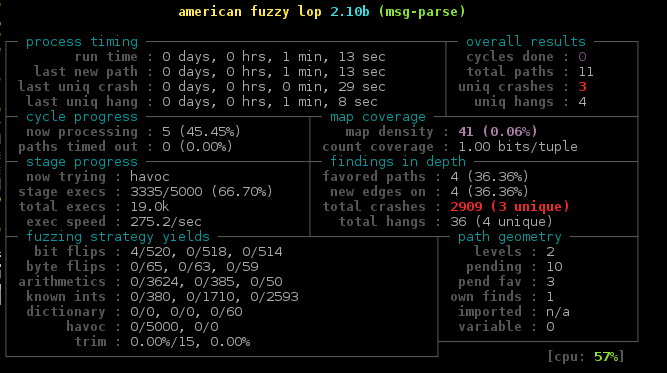
\includegraphics[scale=0.6]{figures/afl-run}
\caption{\texttt{afl} progress screen.}
\label{fig:afl-status}
\end{figure}

\subsection{Results}

\texttt{afl} created 3 unique test cases that pinpointed each memory
safety vulnerability in under 1 minute. \texttt{afl} saved each test case, and
crash uniqueness was confirmed manually using
\texttt{valgrind}\footnote{http://valgrind.org/}.

\subsubsection{A Sample \texttt{afl} Test Case}

Figure \ref{fig:hexdump} shows the hexdump of a sample test case generated by
\texttt{afl}. The highlighted byte,
corresponding to the \texttt{addr\_len} field of the a \texttt{msg\_t} struct,
is set to \texttt{0x9c}, longer than the length of the message.

This triggers vulnerability \texttt{UNSAFE 1} in Line 3 of Figure \ref{fig:vuln-snippet}, causing an attempted read of invalid memory.

\begin{figure}[H]
    \begin{lstlisting}[language={},basicstyle=\small]
     01 (*@\hl{9c}@*) 02 00 23 6e 57 47  59 50 51 49 53 63 57 47
     6c 49 35 71 6b 42 59 4b  4b 36 31 76 58 56 68 73
     6f 57 68\end{lstlisting}
\caption{Hexdump of an \texttt{afl}-generated test file triggering the vulnerability \texttt{UNSAFE 1}}
\label{fig:hexdump}
\end{figure}

See Appendix \ref{app:test-cases} for a listing of each test case \texttt{afl}
generated and the corresponding memory fault uncovered.

\subsection{Overall Evaluation}

\texttt{afl} is extremely easy to use and very high performance. It identified
each memory fault in the test program and produced repeatable test cases
for each unique bug. \texttt{afl} is an outstandingly easy and effective
tool.

\section{\texttt{afl} in the Real World}

\texttt{afl} has had extraordinary success in uncovering both security
vulnerabilities and non-security related bugs in real-world software. Table
\ref{fig:afl-trophies}, a small subset of the \texttt{afl} ``bug-o-rama trophy case''\cite{afl-trophy-case},
shows a handful of famous projects that have had serious security
vulnerabilities uncovered by \texttt{afl}.

\begin{table}[H]
\centering
\begin{tabular}{c | c | c}
libpng & libtiff & mozjpeg \\
PHP & Mozilla Firefox & Internet Explorer \\
Apple Safari & Adobe Flash / PCRE & sqlite \\
OpenSSL & LibreOffice & GnuPG \\
OpenSSH & PuTTY & nginx \\
bash (post-Shellshock) & JavaScriptCore & ffmpeg \\
wireshark & ImageMagick & BIND \\
QEMU & Oracle BerkeleyDB & Android / libstagefright \\
iOS / ImageIO & FLAC audio library & less / lesspipe \\
strings & file & dpkg \\
OpenBSD pfctl & NetBSD bpf & man \\
libxml2 & glibc & clang / llvm \\
redis & perl & curl \\
VLC & screen & tmux  \\
Mozilla NSS & dhcpcd & Linux ext4 \\
\end{tabular}
\caption{A small sample of well-known projects owned by \texttt{afl}}
\label{fig:afl-trophies}
\end{table}

\section{Conclusion}

Due to its raw power and proven effectiveness, \texttt{afl} has become one of
the most important practical security tools in the world today. \texttt{afl}'s
efficient and effective genetic algorithms and combination of fuzzing
strategies make it the best freely-available fuzzing tool, and its ease
of use means that very little prior knowledge is needed to unlock its full
power.

It is a serious mistake to deploy production code without running it through
the \texttt{afl} ringer.
